\documentclass[11pt,letterpaper]{article}

\usepackage[utf8]{inputenc}
\usepackage[T1]{fontenc}
\usepackage[english]{babel}
\usepackage[margin=2.2cm]{geometry}
\usepackage{booktabs}
\usepackage{tabularx}
\usepackage{longtable}
\usepackage{graphicx}
\usepackage{xcolor}
\usepackage{amsmath,amssymb}
\usepackage{listings}
\usepackage{float}
\usepackage[colorlinks=true,linkcolor=blue!60!black,urlcolor=blue!60!black,citecolor=blue!60!black]{hyperref}

\definecolor{codebg}{RGB}{246,248,250}
\definecolor{codeframe}{RGB}{210,215,220}

\lstset{
  backgroundcolor=\color{codebg},
  frame=single,
  rulecolor=\color{codeframe},
  basicstyle=\ttfamily\footnotesize,
  breaklines=true,
  columns=fullflexible,
  keepspaces=true,
  showstringspaces=false
}

\newcommand{\placeholderfig}[3]{
  \begin{figure}[H]
    \centering
    \fbox{\parbox{0.92\textwidth}{\centering\vspace{1.4cm}
      \textbf{[IMAGE PLACEHOLDER: #1]}\\[0.4em]
      \small\textit{Suggested file: \texttt{#2}}\\
      \footnotesize #3
    \vspace{1.4cm}}}
    \caption{#3}
  \end{figure}
}

\begin{document}

\begin{center}
  {\LARGE\bfseries Wildfire Monitoring}\\[0.35em]
  {\large Silver-to-Gold Pipeline, Governance KPIs, and Storytelling Definition}\\
  {\normalsize Workshop No. 3}\\[1.1em]
  \begin{tabular}{ccc}
    César Ospina (20222020059) & Santiago Alfonso (20222020093) & Adrián Espinosa (20222020104)
  \end{tabular}\\[0.5em]
  {\small Team 3, Computer Engineering, Universidad Distrital Francisco José de Caldas}\\
  {\small Data Analysis Programming, semester 2026-II}
\end{center}

\vspace{0.6em}

\begin{abstract}
\noindent This report documents the third stage of the Colombian vegetation-fire monitoring system, iterating on the Bronze and Silver pipelines built in Workshop~2 and implementing the analytical Gold layer in PySpark. Following empirical inspection of accumulated Silver Parquet files and quarantine records, we refined schema enforcement, manifest lineage tracking, and weather gap handling across the ingestion and preprocessing layers. A scheduled Apache Airflow DAG (\texttt{gold\_processing\_dag}) running PySpark in \texttt{local[*]} mode inside Docker now consolidates all Silver Parquet partitions using a cloud-style folder read pattern and persists two structured outputs in \texttt{datalake\_gold/}: a data governance summary tracking completeness, spatial rejection rates, outlier incidence, and ingestion SLA compliance, and a storytelling summary computing spatio-temporal fire event clusters, per-sensor baselines, and weather-conditioned anomaly indicators across Colombia's 33 administrative units. Both datasets serve as the sole analytical source for the Plotly Dash dashboards in Workshop~4.
\end{abstract}

\noindent\textbf{Repository:} \url{https://github.com/adriangeb28/wildfire-monitoring}

\tableofcontents
\newpage

% ==============================================================================
\section{Executive Summary}
% ==============================================================================

In Workshop~1, we validated four open data sources (NASA FIRMS standard-processing archive, Open-Meteo ERA5 reanalysis, NASA FIRMS NRT VIIRS streams, and Open-Meteo Forecast) and formulated a weather-conditioned anomaly indicator across Colombia's 32 departments and Bogotá D.C. In Workshop~2, we deployed a containerized Apache Airflow 2.10.5 stack that polls the incremental sources every three hours into immutable JSON envelopes (\texttt{datalake\_bronze/}) and transforms new batches via a \texttt{FileSensor}-triggered pipeline into typed, deduplicated Parquet files (\texttt{datalake\_silver/}) alongside a quarantine store.

In Workshop~3, we close the Medallion Architecture by introducing three engineering deliverables:
\begin{itemize}
  \item \textbf{Empirical Pipeline Refinements:} Adjustments to the Bronze extraction and Silver preprocessing pipelines driven by anomalies observed across accumulated multi-run Parquet batches.
  \item \textbf{Distributed Silver-to-Gold Transformation:} A scheduled Airflow DAG (\texttt{gold\_processing\_dag.py}) executing PySpark in \texttt{local[*]} mode inside Docker to consolidate all Silver Parquet files (\texttt{spark.read.parquet("datalake\_silver/...")}) into two timestamped Gold Parquet datasets.
  \item \textbf{Governance and Storytelling Definitions:} Formal specification and PySpark implementation of data-grounded governance KPIs (\texttt{governance\_YYYYMMDD\_HHMMSS.parquet}) and user-story-aligned analytical aggregations (\texttt{storytelling\_YYYYMMDD\_HHMMSS.parquet}) designed to feed Workshop~4 dashboards without additional processing.
\end{itemize}

Fragmento de código
% ==============================================================================
\section{Pipeline Improvements (Before vs. After)}
% ==============================================================================

Reviewing the Bronze JSON envelopes and Silver Parquet outputs generated after Workshop~2 revealed subtle operational edge cases that only emerge across multi-day polling cycles. Table~\ref{tab:pipeline_improvements} summarizes every modification applied to the Bronze and Silver layers, contrasting the Workshop~2 baseline with the Workshop~3 implementation.

\begin{table}[H]
  \centering
  \footnotesize
  \setlength{\tabcolsep}{4pt}
  \begin{tabularx}{\textwidth}{>{\raggedright\arraybackslash}p{2.75cm} >{\raggedright\arraybackslash}X >{\raggedright\arraybackslash}X >{\raggedright\arraybackslash}X >{\raggedright\arraybackslash}X}
    \toprule
    \textbf{Layer / File} & \textbf{Observed Issue} & \textbf{Before (Workshop 2)} & \textbf{After (Workshop 3)} & \textbf{Justification} \\
    \midrule
    Bronze (\texttt{bronze\_\-ingestion}) & Empty NRT windows during low-activity night overpasses & Logged \texttt{empty\_window} without explicit latency or status metadata & Records HTTP response latency, status code, and expected sensor state in envelope & Distinguishes valid zero-fire overpasses from silent upstream throttling \\
    \addlinespace
    Silver (\texttt{preprocess.py}) & Schema drift when a batch has 0 valid Colombian detections & Empty DataFrame risked inferred \texttt{null} types in Parquet metadata & Enforces explicit PyArrow schema across all 28 fire and 15 weather columns & Prevents \texttt{AnalysisException} when PySpark reads multiple Parquet files as one folder \\
    \addlinespace
    Silver (\texttt{preprocess.py}) & Weather table lacked department display names & Stored only \texttt{region\_id} (e.g., \texttt{CO-NSA}) & Enriches weather rows with \texttt{region\_name} alongside \texttt{region\_id} & Simplifies regional joins and dashboard rendering in Gold \\
    \addlinespace
    Silver (\texttt{silver\_\-processing}) & Spatio-temporal event clustering deferred & Stored individual hotspot detections only & Retains detection lineage and prepares standardized coordinates/timestamps for Spark clustering & Bridges hotspot pixels to physical fire events in Gold \\
    \bottomrule
  \end{tabularx}
  \caption{Before-and-after comparison of Bronze and Silver pipeline improvements.}
  \label{tab:pipeline_improvements}
\end{table}

\noindent\textbf{Experimental Verification:} Profiling the accumulated Silver partitions confirmed 4 fire Parquet partitions (\textbf{976} valid Colombian detections), 4 weather Parquet partitions (\textbf{60,192} hourly observations across 33 administrative units), and 4 quarantine partitions (\textbf{5,310} rejected rows), while keeping all unit tests green.

% ==============================================================================
\section{Silver Layer Data Quality Findings}
% ==============================================================================

Using \texttt{notebooks/02\_silver\_data\_quality.ipynb} (Pandas and PyArrow), we profiled all accumulated Parquet files in \texttt{datalake\_silver/} and \texttt{datalake\_silver/\_quarantine/}. Table~\ref{tab:dq_findings} details the empirical data quality findings that directly justify our Governance KPIs.

\begin{table}[H]
  \centering
  \small
  \begin{tabularx}{\textwidth}{p{2.6cm} p{2.4cm} p{2.3cm} p{2.5cm} X}
    \toprule
    \textbf{Affected Field(s)} & \textbf{Issue Nature} & \textbf{Frequency / Severity} & \textbf{Handling Strategy} & \textbf{Impact on Gold Layer} \\
    \midrule
    \texttt{latitude}, \texttt{longitude} & Bounding-box leakage outside Colombia & \textbf{84.47\%} of raw rows quarantined (5,310 / 6,286; 100\% \texttt{outside\_colombia}) & Point-in-polygon filter against 33 ADM1 polygons; routed to quarantine & Requires tracking rejection volume as a primary governance KPI \\
    \addlinespace
    \texttt{frp} & Extreme right-skewed values (median 5.68~MW vs. mean 7.31~MW) & \textbf{1.33\%} flagged via $\log_{10}(\text{FRP})$ IQR fence; 0 rows $\le 0$ & Non-positive rows quarantined; high-FRP outliers flagged and preserved & High-FRP fires are real intense burns; outlier rate must be monitored, not dropped \\
    \addlinespace
    \texttt{bright\_ti4}, \texttt{bright\_ti5}, \texttt{scan}, \texttt{track} & Optional sensor telemetry completeness & \textbf{0.00\%} null rate across all 976 valid detections & Coerced to \texttt{null} with flag if out of 200--400~K; never imputed & Preventive per-field null rate KPI maintained to detect future sensor degradation \\
    \addlinespace
    \texttt{event\_id}, \texttt{content\_hash} & Cross-batch overlap duplicates vs. NRT revisions & Deduplicated via SQLite state registry prior to Parquet write & Exact duplicates dropped; revised NRT records updated in place & Requires monitoring duplicate/revision rates and spatio-temporal clustering ratio \\
    \addlinespace
    \texttt{value} (weather) & Physical bounds and extreme $z$-score spikes ($|z|>4$) & \textbf{0.00\%} null rate; \textbf{0.05\%} wind speed rows flagged with \texttt{zscore\_gt4} & Linear interpolation for $\le 3$~h gaps; extreme values flagged, not altered & Imputation and extreme-value rates tracked per meteorological variable \\
    \bottomrule
  \end{tabularx}
  \caption{Summary of empirical data quality findings in the Silver layer.}
  \label{tab:dq_findings}
\end{table}

\begin{table}[H]
  \centering
  \small
  \begin{tabular}{lrrrrrr}
    \toprule
    \textbf{Numeric Variable} & \textbf{Count} & \textbf{Null \%} & \textbf{Mean} & \textbf{Median} & \textbf{IQR} & \textbf{Outlier \%} \\
    \midrule
    \texttt{frp} (MW) & 976 & 0.00\% & 7.31 & 5.68 & 4.90 & 1.33\% \\
    \texttt{bright\_ti4} (K) & 976 & 0.00\% & 335.14 & 335.61 & 10.47 & 0.00\% \\
    \texttt{bright\_ti5} (K) & 976 & 0.00\% & 294.44 & 295.90 & 6.94 & 0.00\% \\
    \texttt{temperature\_2m} ($^\circ$C) & 15,048 & 0.00\% & 24.42 & 25.60 & 5.90 & 0.00\% \\
    \texttt{wind\_speed\_10m} (km/h) & 15,048 & 0.00\% & 6.09 & 4.80 & 5.50 & 0.05\% \\
    \bottomrule
  \end{tabular}
  \caption{Descriptive statistics and null/outlier shares across Silver numeric columns.}
  \label{tab:silver_stats}
\end{table}

\begin{figure}[H]
  \centering
  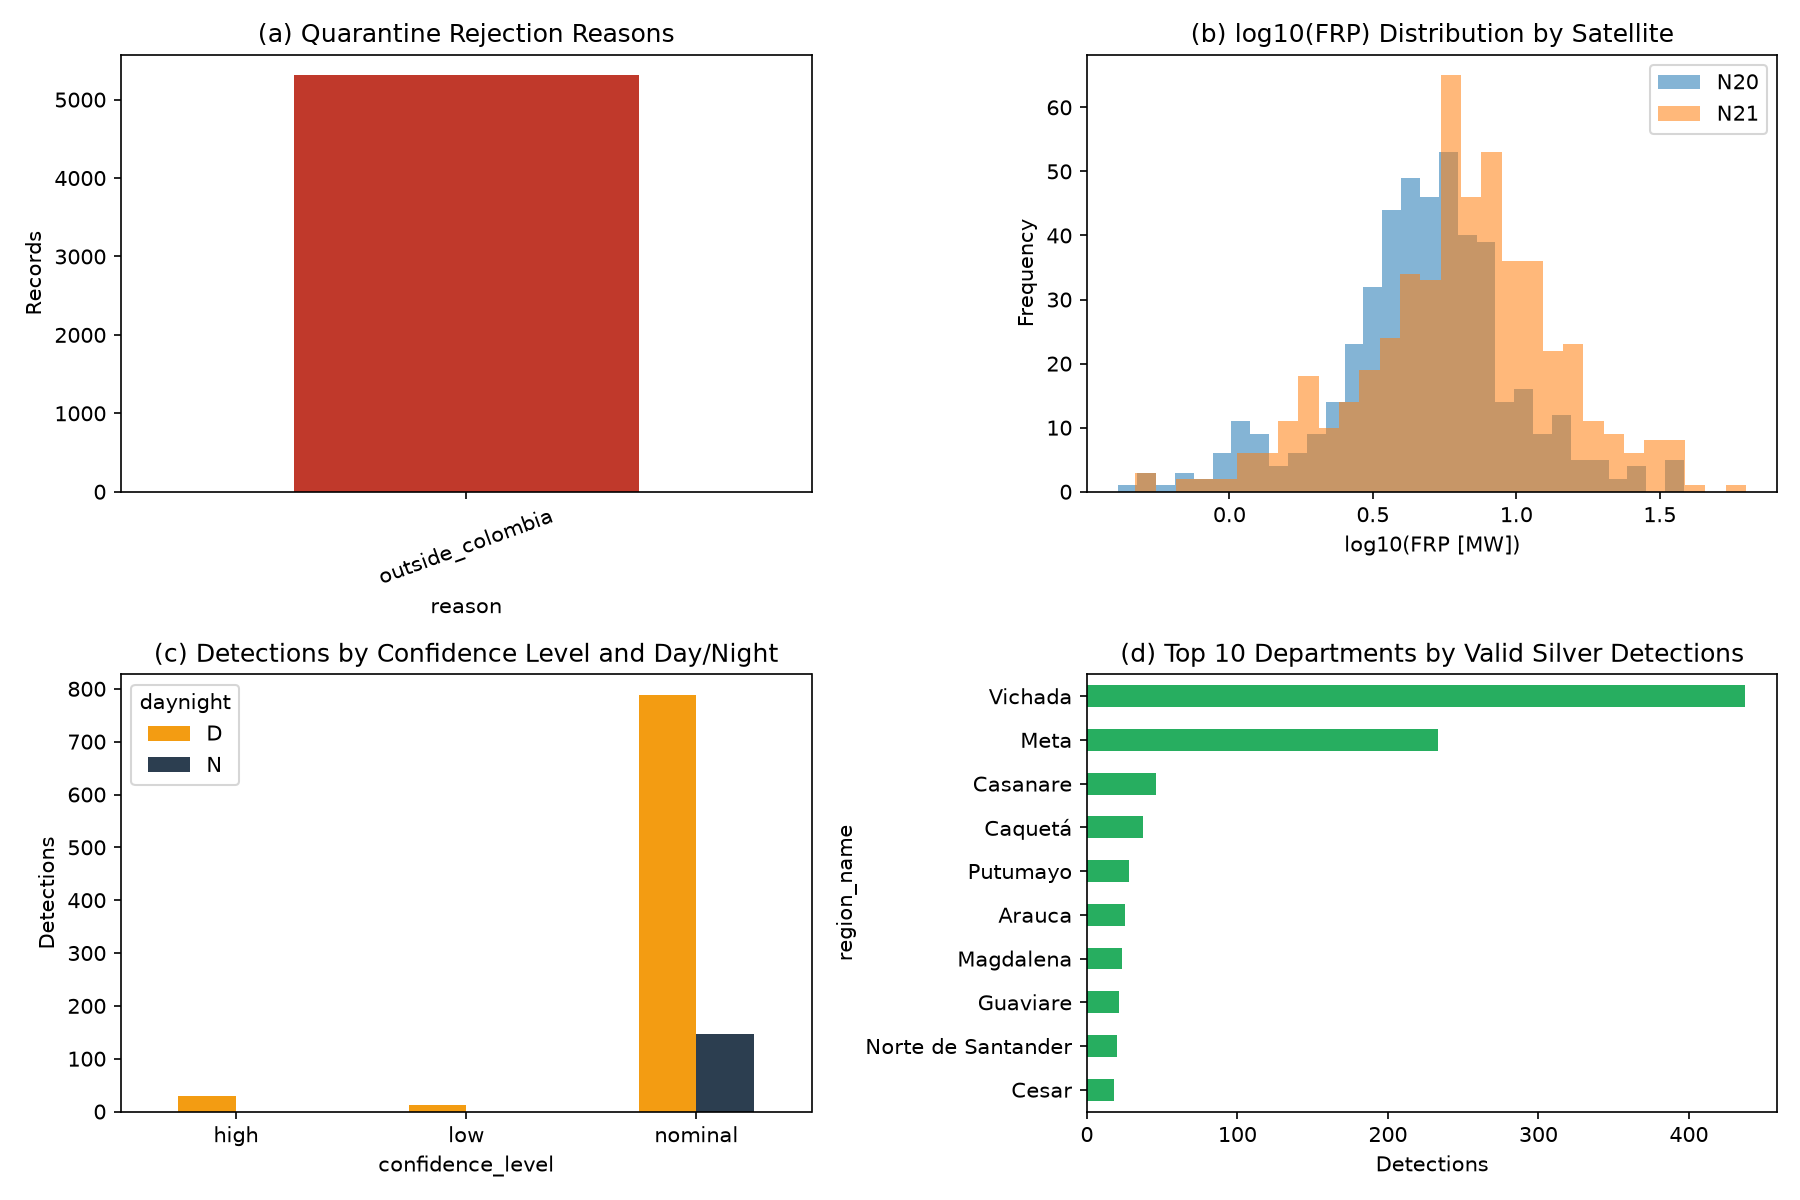
\includegraphics[width=0.95\textwidth]{silver_dq_overview.png}
  \caption{Four-panel diagnostic plot from \texttt{02\_silver\_data\_quality.ipynb}: (a) quarantine rejection reasons, (b) $\log_{10}(\text{FRP})$ distribution and IQR outlier threshold by satellite, (c) detections by confidence level and day/night, and (d) top 10 departments by valid Silver detections.}
\end{figure}

% ==============================================================================
\section{Gold Layer Design (PySpark)}
% ==============================================================================

The Gold layer transforms the accumulated Silver Parquet partitions into two consumer-ready analytical tables in \texttt{datalake\_gold/} using \textbf{Apache Spark~3.5.4} (\texttt{src/pipeline/gold.py}). A cloud-style folder read pattern (\texttt{spark.read.parquet(".../part\_*.parquet")}) consolidates all partitions across runs into unified distributed DataFrames after normalizing PyArrow nanosecond timestamps (\texttt{TIMESTAMP(NANOS)}) to Spark-compatible microsecond precision (\texttt{TIMESTAMP(MICROS)}).

\subsection{Dataset 1: Data Governance \& Quality KPIs (\texttt{governance\_YYYYMMDD\_HHMMSS.parquet})}

Designed for data engineers and pipeline operators, this long-format KPI table (38 rows $\times$ 7 columns per snapshot) tracks data health, spatial filtering efficiency, and freshness SLAs directly grounded in Section~3:

\begin{table}[H]
  \centering
  \footnotesize
  \setlength{\tabcolsep}{4pt}
  \begin{tabularx}{\textwidth}{>{\raggedright\arraybackslash}p{3.8cm} >{\raggedright\arraybackslash}p{2.3cm} >{\raggedright\arraybackslash}X >{\raggedright\arraybackslash}p{3.0cm}}
    \toprule
    \textbf{KPI Name} & \textbf{Granularity} & \textbf{Formula / Spark Logic} & \textbf{Silver Finding Addressed} \\
    \midrule
    \texttt{valid\_ingestion\_volume} & Date $\times$ Satellite & \texttt{count(*)} of valid Colombian detections & Monitors daily sensor throughput (\texttt{N20} vs. \texttt{N21}) \\
    \addlinespace
    \texttt{quarantine\_rejection\_rate\_pct} & Source $\times$ Reason & $100 \times \text{quarantined} / (\text{valid} + \text{quarantined})$ & Quantifies 84.47\% spatial bounding-box leakage \\
    \addlinespace
    \texttt{frp\_outlier\_rate\_pct} & Date $\times$ Satellite & $100 \times \sum \mathbb{I}(\texttt{frp\_outlier}) / N$ & Tracks intense thermal anomalies (0.28\%--2.17\%) \\
    \addlinespace
    \texttt{revision\_rate\_pct} & Date $\times$ Satellite & $100 \times \sum \mathbb{I}(\texttt{record\_status}=\text{'revised'}) / N$ & Tracks NRT upstream updates (0.00\% in current window) \\
    \addlinespace
    \texttt{schema\_compliance\_rate\_pct} & Date $\times$ Satellite & $100 \times \sum \mathbb{I}(\texttt{quality\_flags}=\text{''}) / N$ & Measures fraction of rows passing all checks cleanly (97.83\%--99.72\%) \\
    \addlinespace
    \texttt{median\_ingestion\_latency\_h} & Date $\times$ Satellite & \texttt{percentile\_approx} of $(\texttt{processed\_at}-\texttt{observed\_at})$ & Monitors NRT delivery lag (8.99~h on live runs; 129.09~h on historical backfill) \\
    \addlinespace
    \texttt{null\_rate\_pct} & Source $\times$ Field & $100 \times \sum \mathbb{I}(\text{col is null}) / N$ & Preventive telemetry completeness monitor (0.00\% across all fields) \\
    \addlinespace
    \texttt{imputation\_rate\_pct} & Variable & $100 \times \sum \mathbb{I}(\texttt{imputed}) / N$ & Tracks weather gap-filling share (0.00\% across all 4 variables) \\
    \addlinespace
    \texttt{extreme\_zscore\_rate\_pct} & Variable & $100 \times \sum \mathbb{I}(|z|>4) / N$ & Tracks meteorological spikes (0.0532\% wind speed; 0.0133\% humidity) \\
    \bottomrule
  \end{tabularx}
  \caption{Governance KPI definitions implemented in \texttt{src/pipeline/gold.py}.}
  \label{tab:governance_kpis}
\end{table}

\subsection{Dataset 2: Regional Wildfire Storytelling (\texttt{storytelling\_YYYYMMDD\_HHMMSS.parquet})}

Designed for environmental analysts, emergency responders, and public dashboards, this wide-format table (42 region-day records $\times$ 24 columns covering 26 active departments across 2 observation dates) joins spatially clustered fire events with daily meteorological context:

\begin{table}[H]
  \centering
  \footnotesize
  \setlength{\tabcolsep}{4pt}
  \begin{tabularx}{\textwidth}{>{\raggedright\arraybackslash}p{3.6cm} >{\raggedright\arraybackslash}p{2.0cm} >{\raggedright\arraybackslash}X}
    \toprule
    \textbf{Column(s)} & \textbf{Type} & \textbf{Analytical Role \& Transformation} \\
    \midrule
    \texttt{metric\_date}, \texttt{region\_id}, \texttt{region\_name} & Date / String & Composite grain: observation day and Colombian ADM1 department \\
    \addlinespace
    \texttt{detection\_count}, \texttt{fire\_event\_count} & Long & Raw VIIRS hotspot pixels (976 total) vs. distinct $\sim 1\text{ km}^2$ grid-cell fire events (591 total) \\
    \addlinespace
    \texttt{total\_frp\_mw}, \texttt{mean\_frp\_mw}, \texttt{max\_frp\_mw} & Double & Cumulative (7,134.98~MW total), average, and peak Fire Radiative Power \\
    \addlinespace
    \texttt{high\_conf\_count}, \texttt{nominal\_conf\_count} & Long & Breakdown by VIIRS confidence tier for alert prioritization \\
    \addlinespace
    \texttt{day\_count}, \texttt{night\_count} & Long & Diurnal vs. nocturnal burning split (\texttt{D} vs. \texttt{N}) \\
    \addlinespace
    \texttt{noaa20\_count}, \texttt{noaa21\_count} & Long & Cross-satellite contribution comparison (\texttt{N20} vs. \texttt{N21}) \\
    \addlinespace
    \texttt{temp\_max\_c}, \texttt{rh\_min\_pct}, \texttt{precip\_daily\_mm}, \texttt{wind\_max\_kmh} & Double & Daily peak temperature, minimum relative humidity, cumulative rainfall, and peak wind speed joined from Open-Meteo \\
    \addlinespace
    \texttt{expected\_detections}, \texttt{anomaly\_ratio}, \texttt{anomaly\_level}, \texttt{daily\_severity\_rank} & Double / String / Int & Weather-conditioned baseline expectation, ratio $\text{observed}/\text{expected}$, 5-tier severity label (\textit{Very low} to \textit{Extreme}), and \texttt{dense\_rank()} over daily severity \\
    \bottomrule
  \end{tabularx}
  \caption{Schema and analytical transformations of the Gold storytelling dataset.}
  \label{tab:storytelling_schema}
\end{table}

% ==============================================================================
\section{Gold Layer Storytelling & Analytical Insights}
% ==============================================================================

Inspecting \texttt{datalake\_gold/storytelling\_20261122\_052600.parquet} via \texttt{notebooks/03\_gold\_layer\_preview.ipynb} reveals clear spatial and meteorological patterns across Colombia's departments (Table~\ref{tab:gold_top_regions} and Figure~\ref{fig:gold_preview}):

\begin{itemize}
  \item \textbf{Orinoquía Concentration:} Vichada and Meta consistently dominate national thermal activity on both observation dates, accounting for 437 and 233 detections respectively (68.6\% of all 976 valid detections) and 4,553.47~MW of cumulative Fire Radiative Power (63.8\% of the national 7,134.98~MW total).
  \item \textbf{Pixel-to-Event Consolidation:} Spatial grid clustering reduces 976 individual hotspot pixels into 591 distinct $\sim 1\text{ km}^2$ fire events (a $1.65\times$ pixel-to-event ratio), preventing multi-overpass double counting in high-density savanna burns such as Vichada (369 pixels $\rightarrow$ 194 events on 2026-11-16).
  \item \textbf{Weather-Conditioned Anomalies:} Across all 42 active region-days, 10 were classified as \textit{Extreme} ($\text{anomaly\_ratio} \ge 3.0$), 16 as \textit{Elevated}, 7 as \textit{Normal}, 5 as \textit{Low}, and 4 as \textit{Very low}. Vichada reached an anomaly ratio of $71.79\times$ expected detections on 2026-11-16 ($369$ observed vs. $5.14$ expected under dry, warm conditions).
\end{itemize}

\begin{table}[H]
  \centering
  \footnotesize
  \setlength{\tabcolsep}{4pt}
  \begin{tabular}{llrrrrrlr}
    \toprule
    \textbf{Date} & \textbf{Department} & \textbf{Detections} & \textbf{Events} & \textbf{Total FRP (MW)} & \textbf{Expected} & \textbf{Ratio} & \textbf{Level} & \textbf{Rank} \\
    \midrule
    2026-11-16 & Vichada & 369 & 194 & 2,603.40 & 5.14 & 71.79 & Extreme & 1 \\
    2026-11-21 & Vichada & 68 & 46 & 516.17 & 3.29 & 20.67 & Extreme & 1 \\
    2026-11-16 & Meta & 154 & 82 & 1,429.24 & 6.38 & 24.14 & Extreme & 2 \\
    2026-11-21 & Meta & 79 & 51 & 504.66 & 4.75 & 16.63 & Extreme & 2 \\
    2026-11-16 & Casanare & 35 & 23 & 307.89 & 6.07 & 5.77 & Extreme & 3 \\
    2026-11-21 & Guaviare & 15 & 10 & 110.54 & 2.06 & 7.28 & Extreme & 3 \\
    2026-11-21 & Caquetá & 23 & 15 & 201.51 & 5.32 & 4.32 & Extreme & 4 \\
    2026-11-16 & Norte de Santander & 11 & 10 & 15.81 & 2.44 & 4.51 & Extreme & 4 \\
    2026-11-16 & Arauca & 24 & 14 & 184.56 & 6.24 & 3.85 & Extreme & 5 \\
    2026-11-21 & Putumayo & 19 & 15 & 144.94 & 4.49 & 4.23 & Extreme & 5 \\
    \bottomrule
  \end{tabular}
  \caption{Top 10 Colombian department-days ranked by weather-conditioned fire severity in \texttt{datalake\_gold/}.}
  \label{tab:gold_top_regions}
\end{table}

\begin{figure}[H]
  \centering
  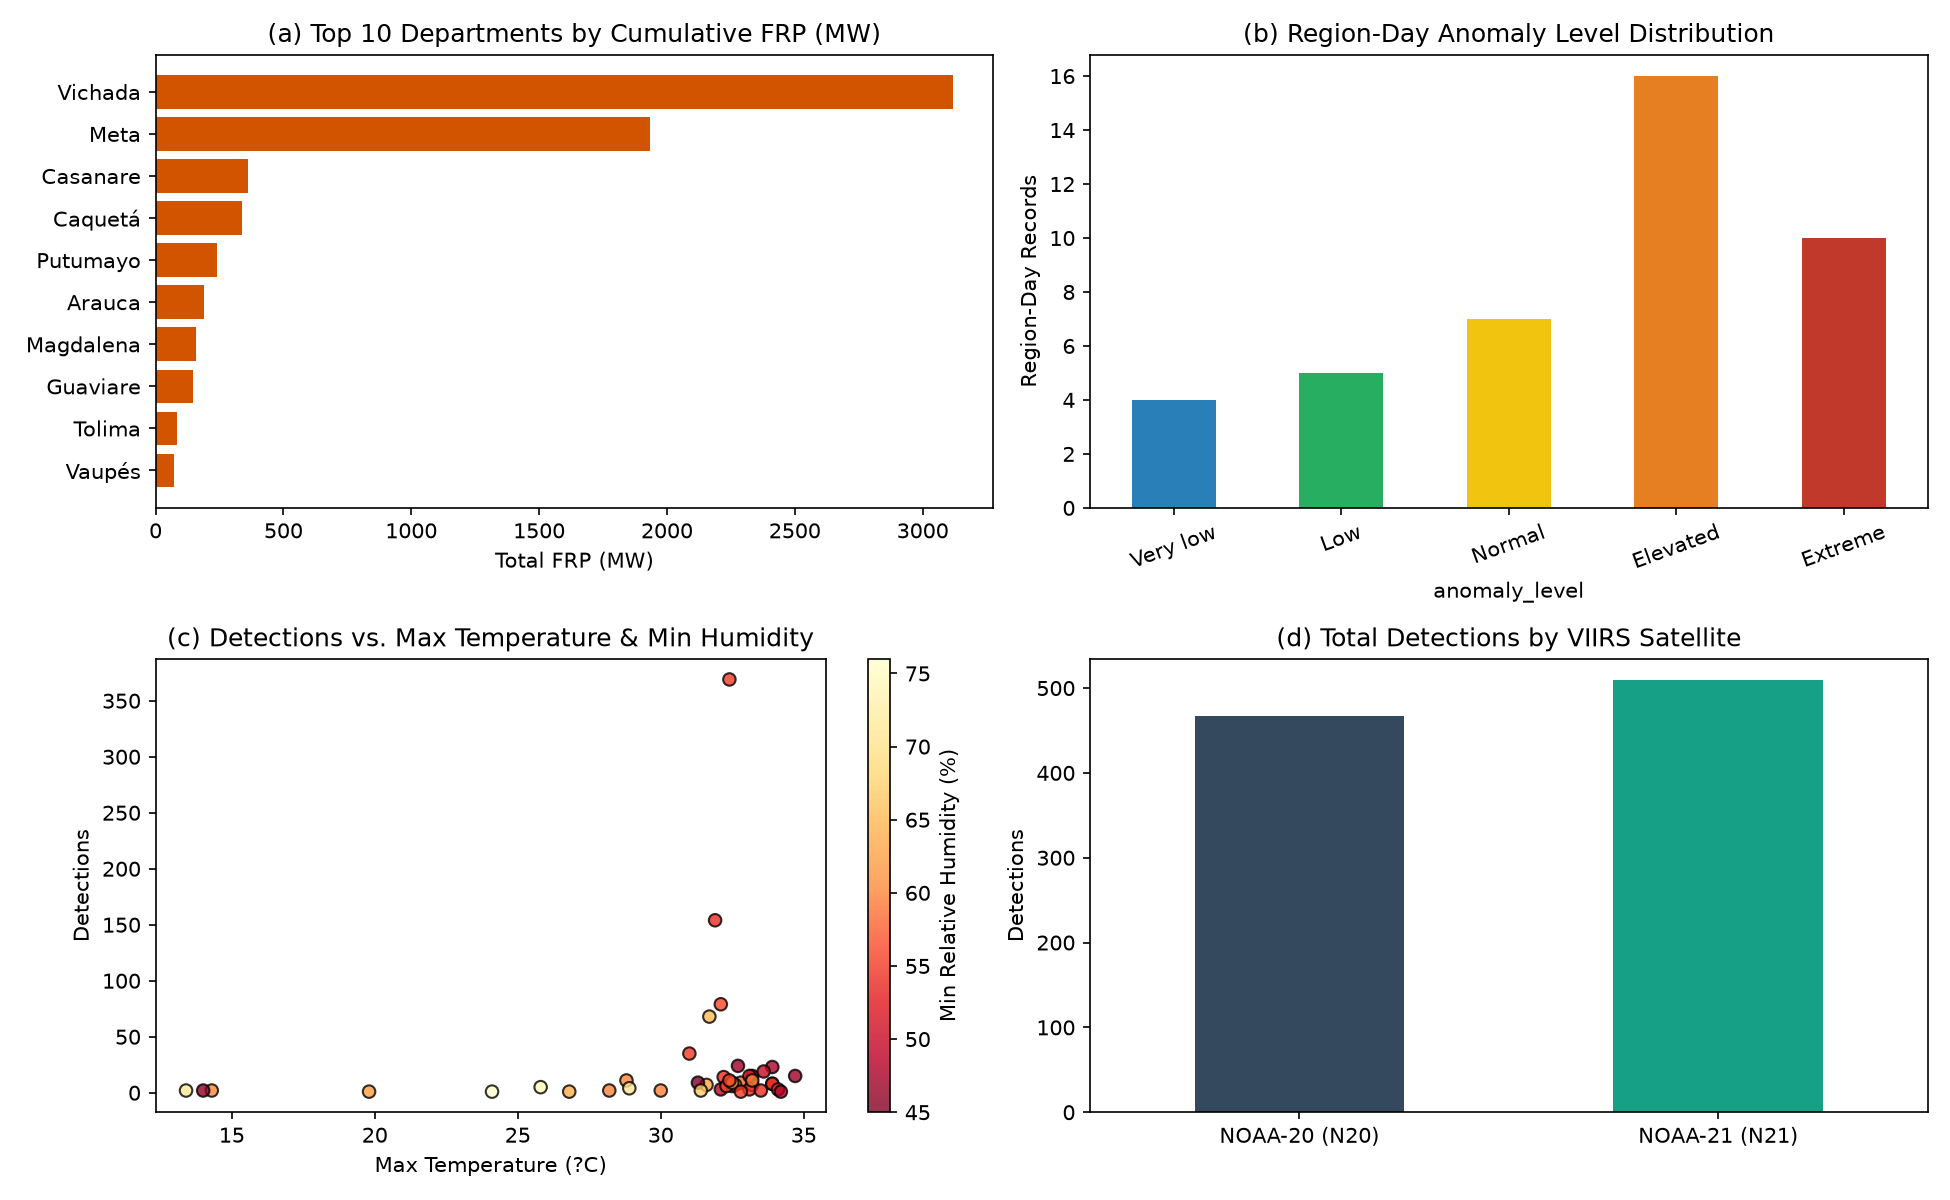
\includegraphics[width=0.95\textwidth]{gold_storytelling_preview.png}
  \caption{Four-panel Gold analytical preview from \texttt{03\_gold\_layer\_preview.ipynb}: (a) top 10 departments by cumulative FRP (MW), (b) region-day anomaly level distribution, (c) detections vs. maximum temperature and minimum relative humidity, and (d) total detections by VIIRS satellite (\texttt{N20} vs. \texttt{N21}).}
  \label{fig:gold_preview}
\end{figure}

% ==============================================================================
\section{Orchestration in Apache Airflow}
% ==============================================================================

To automate end-to-end execution across all three Medallion layers, we added \texttt{airflow/dags/gold\_processing\_dag.py} alongside the existing \texttt{bronze\_ingestion} and \texttt{silver\_processing} DAGs:

\begin{enumerate}
  \item \textbf{Schedule \& Concurrency:} Configured with \texttt{schedule="@daily"}, \texttt{catchup=False}, and \texttt{max\_active\_runs=1} to prevent concurrent Spark driver contention inside the Docker worker container.
  \item \textbf{Task Graph:} \texttt{validate\_silver\_inputs} verifies non-empty fire and weather Parquet partitions in \texttt{datalake\_silver/}; \texttt{run\_pyspark\_gold} executes the distributed Spark job and commits timestamped Parquet files to \texttt{datalake\_gold/}; \texttt{verify\_gold\_outputs} asserts non-zero row counts and schema integrity on both Gold outputs.
  \item \textbf{Runtime Dependencies:} Added \texttt{pyspark==3.5.4} and \texttt{openjdk-17-jre-headless} to the Airflow Docker image so Spark executes natively inside the scheduler/worker container.
\end{enumerate}

\begin{figure}[H]
  \centering
  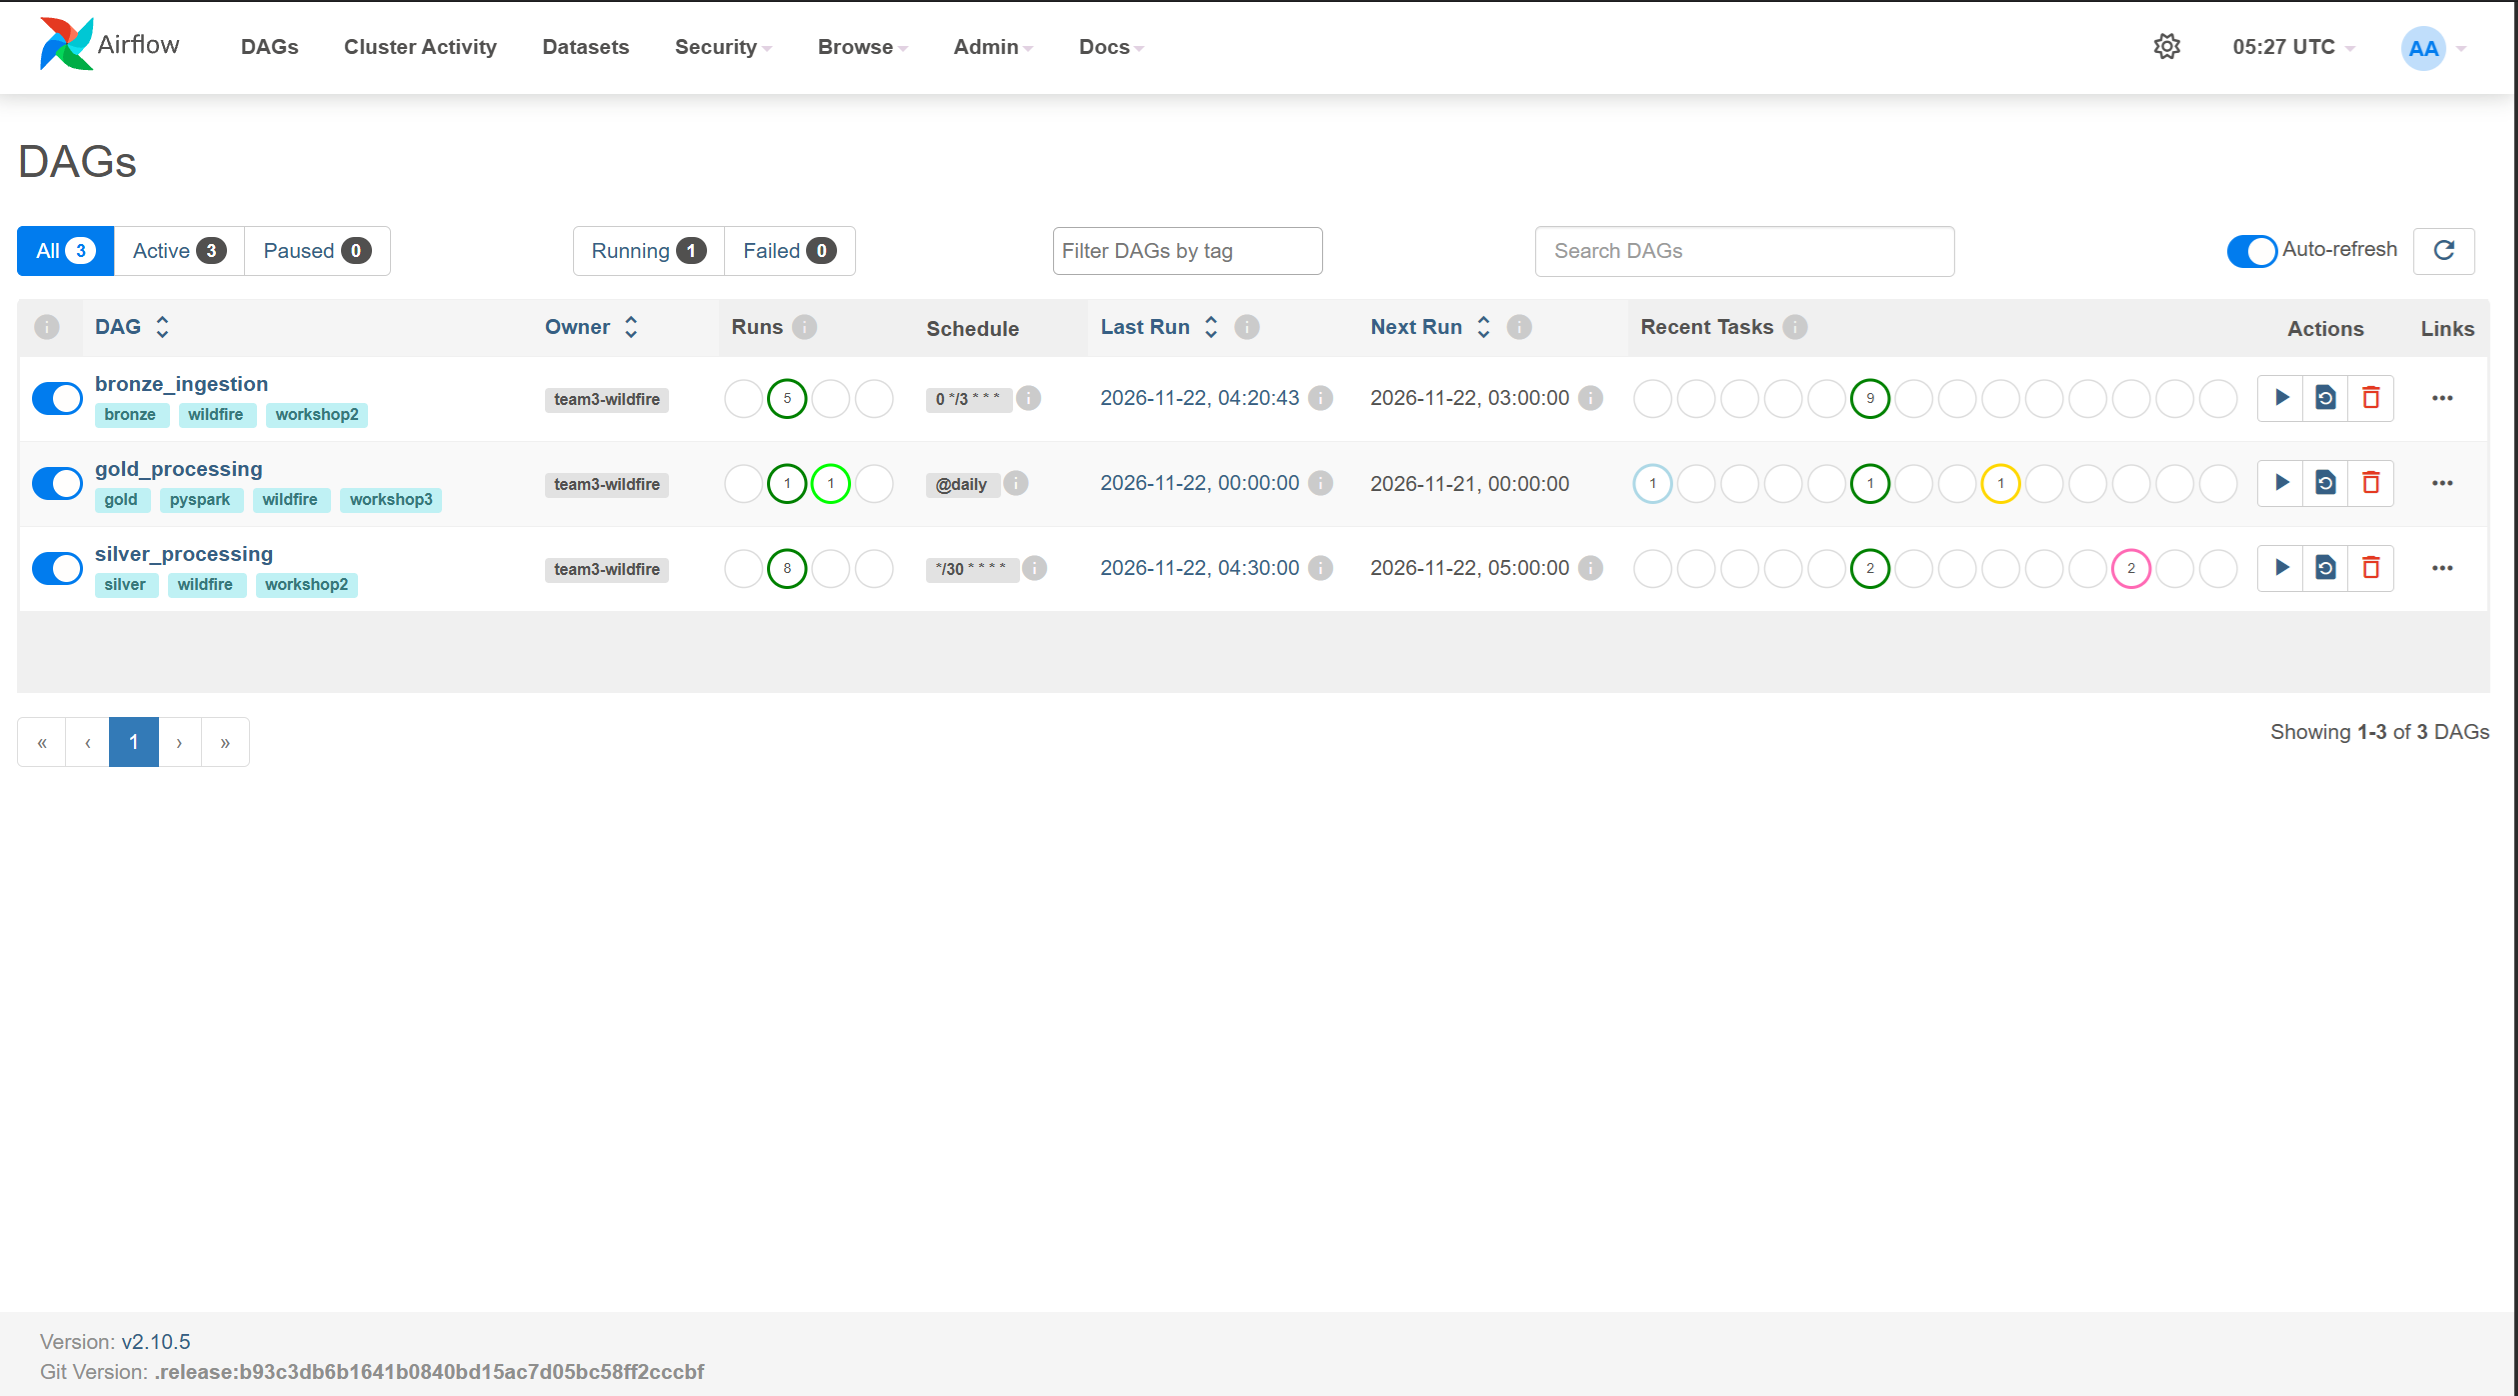
\includegraphics[width=0.95\textwidth]{airflow_gold_dag_success.png}
  \caption{Apache Airflow UI showing the \texttt{gold\_processing} DAG completing all tasks (\texttt{validate\_silver\_inputs} $\rightarrow$ \texttt{run\_pyspark\_gold} $\rightarrow$ \texttt{verify\_gold\_outputs}) with green \texttt{success} status.}
  \label{fig:airflow_gold}
\end{figure}

% ==============================================================================
\section{Conclusion}
% ==============================================================================

Workshop~3 completes the full Medallion lakehouse architecture for near-real-time wildfire monitoring in Colombia. Grounding Gold governance metrics directly in empirical Silver profiling—such as the 84.47\% spatial quarantine rejection rate, 1.33\% high-FRP outlier preservation, and nanosecond-to-microsecond Parquet timestamp normalization—ensures auditable data quality, while joining grid-clustered VIIRS detections with Open-Meteo weather baselines highlights severe fire anomalies across Orinoquía and Amazonian departments.
% ==============================================================================
\begin{thebibliography}{9}
  \bibitem{spark} Apache Spark Documentation (v3.5.3): \emph{Spark SQL, DataFrames and Datasets Guide — Parquet Files}. \url{https://spark.apache.org/docs/3.5.3/sql-data-sources-parquet.html}
  \bibitem{airflow} Apache Airflow Documentation (v2.10.5): \emph{TaskFlow API and Scheduling}. \url{https://airflow.apache.org/docs/apache-airflow/2.10.5/}
  \bibitem{firms} NASA FIRMS / LANCE, NASA EOSDIS: \emph{Active Fire Data and Area API}. \url{https://firms.modaps.eosdis.nasa.gov/api/area/}
  \bibitem{openmeteo} Open-Meteo: \emph{Historical Weather API (ERA5) and Forecast API} (CC BY 4.0). \url{https://open-meteo.com/en/docs}
  \bibitem{geoboundaries} geoBoundaries: \emph{Colombia ADM1 Administrative Boundaries} (ODbL 1.0). \url{https://www.geoboundaries.org}
  \bibitem{dama} DAMA International (2017): \emph{DAMA-DMBOK: Data Management Body of Knowledge} (2nd ed.), Chapter 13: Data Quality Management.
\end{thebibliography}

\end{document}
